\begin{frame}
  \frametitle{Hanging nodes}
\end{frame}

\begin{frame}
  \frametitle{Hanging nodes}
\vspace{-2.0cm}
  \begin{itemize}
    \item Regular mesh\\[2mm]    
    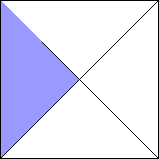
\includegraphics[height=0.3\textheight]{regular_a}
  \end{itemize}
\end{frame}

\begin{frame}
\vspace{-2.0cm}
  \frametitle{Hanging nodes}
  \begin{itemize}
    \item Regular mesh\\[2mm]    
    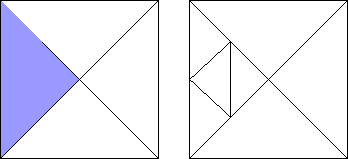
\includegraphics[height=0.3\textheight]{regular_b}
  \end{itemize}
\end{frame}

\begin{frame}
\vspace{-2.0cm}
  \frametitle{Hanging nodes}
  \begin{itemize}
    \item Regular mesh\\[2mm]    
    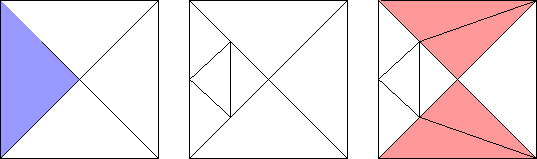
\includegraphics[height=0.3\textheight]{regular_c}
  \end{itemize}
\end{frame}

\begin{frame}
  \frametitle{Hanging nodes}
  \begin{itemize}
    \item Regular mesh\\[2mm]    
    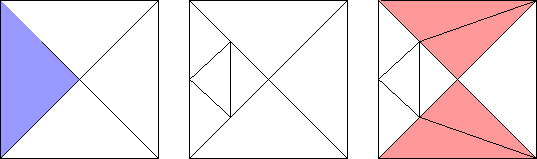
\includegraphics[height=0.3\textheight]{regular_c}
    \item One-level hanging nodes (1-irregular mesh)\\[2mm]   
    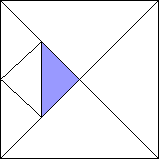
\includegraphics[height=0.3\textheight]{one_irr_a}
  \end{itemize}
\end{frame}

\begin{frame}
  \frametitle{Hanging nodes}
  \begin{itemize}
    \item Regular mesh\\[2mm]    
    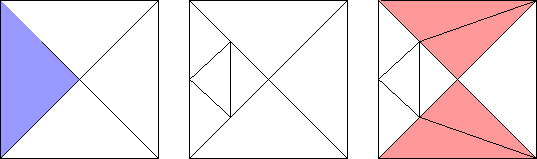
\includegraphics[height=0.3\textheight]{regular_c}
    \item One-level hanging nodes (1-irregular mesh)\\[2mm]   
    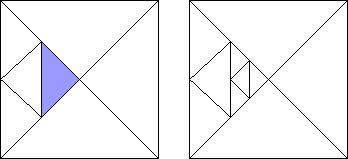
\includegraphics[height=0.3\textheight]{one_irr_b}
  \end{itemize}
\end{frame}

\begin{frame}
  \frametitle{Hanging nodes}
  \begin{itemize}
    \item Regular mesh\\[2mm]    
    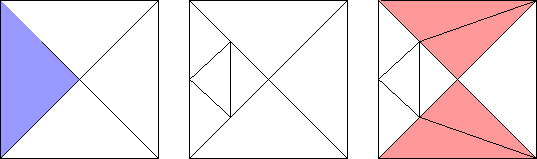
\includegraphics[height=0.3\textheight]{regular_c}
    \item One-level hanging nodes (1-irregular mesh)\\[2mm]
    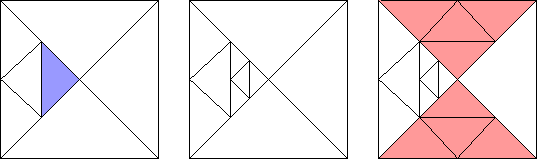
\includegraphics[height=0.3\textheight]{one_irr_c}
  \end{itemize}
\end{frame} 
